\documentclass[9pt]{article}

\usepackage{graphicx,epsfig,psfrag,rotate,xcolor,url}
\usepackage{amsmath,amsfonts,amssymb,latexsym,multicol}
\usepackage{setspace,enumerate,enumitem,ifthen,subfig}
\usepackage{hyperref,framed,enumitem,tikz}
\usepackage{svg}
\usepackage{float}
\usepackage{siunitx,tcolorbox}
\usepackage[portuges]{babel}
\usepackage[utf8]{inputenc}
\usepackage[algo2e,english,onelanguage,algoruled]{algorithm2e}
\usepackage[margin=0.5in]{geometry}
\usepackage{calrsfs,empheq}
\renewcommand{\rmdefault}{pplx}
\usepackage{eulervm}
\DeclareMathAlphabet{\mathcal}{OMS}{zplm}{m}{n}
\usepackage{minted}


\newcommand{\R}{\mathbb{R}}
\newcommand{\N}{\mathbb{N}}
\newcommand{\C}{\mathbb{C}}
\newcommand{\F}{\mathbb{F}}
\renewcommand{\d}{\mathrm{d}}
\newcommand{\V}{\mathbb{V}}
\renewcommand{\P}{\mathbb{P}}
\newcommand{\spn}{\mathbf{span}\,}
\DeclareMathOperator*{\argmin}{argmin}

\hypersetup{
    colorlinks=true,
    linkcolor=magenta,
    filecolor=magenta,      
    urlcolor=cyan,
    }

\definecolor{mygray}{RGB}{248,248,250}
\newcommand*\mymathbox[1]{%
  \fcolorbox{black}{mygray}{\hspace{1em}#1\hspace{1em}}}

\begin{document}
%\hrule

\begin{tcolorbox}[colframe=black,colback=gray!20,arc=0pt]
\begin{center}
{\sc\LARGE EE400 -- Métodos da Engenharia Elétrica} \vspace{0.5cm}
\hrule \vspace{0.2cm}
{\large \begin{tabular}{c|c}
\begin{tabular}{l} Projeto D: GNSS e Drones\end{tabular} & \begin{tabular}{l} João Felipe Contreras De Moraes \\ {\tt j174140@dac.unicamp.br} \end{tabular}
\end{tabular}}
\end{center}
\end{tcolorbox}

\vspace{0.3cm}

%\begin{multicols}{2}

\noindent
\begin{tcolorbox}[colframe=black,width =7cm,colback=gray!20,arc=0pt]
\centering {\sc {\bf Introdução}}
\end{tcolorbox}

\vspace{0.3cm}

O \textbf{GPS} (\textit{Global Positioning System}) é um sistema de posicionameto por rádio baseado em satélites. A sigla já faz parte do cotidiano quando deseja-se referir a um sistema de navegação por satélites capaz de determinar a posição de um receptor ou uma base de tempo, pois estão presentes nos smartphones, automóveis, na aviação e, em particular, na navegação de drones.

No entanto, o GPS é apenas uma instância de um \textbf{sistema de navegação por satélite} (GNSS) que pertence ao governo dos Estados Unidos. Atualmente existem  3 outros sistemas operacionais, além do americano: GLONASS (Rússia), BeiDou (China) e Galileo (União Europeia). Sendo que Índia também tem planos de expandir seu sistema regional (IRNSS) para escala global. O alcance global desses sistemas é obtido a partir de uma constelação com até 30 satélites em órbitas médias ($R\approx 20000\ \text{km}$) distribuídas em diferentes planos.

Os sistemas de posicionamento por rádio de forma geral são formados por um conjunto de transmissores e receptores. No caso do GNSS, o receptor pode ser visto como uma antena cuja posição desejamos determinar e os transmissores são os satélites de uma determina constelação. Os satélites transmitem sinais na banda L (frequência de 1-2 GHz), que codificam informações para determinar o tempo de envio do sinal, dados das órbitas, informações de calibração, entre outros. O receptor, com um relógio interno, é capaz de determinar o tempo de recebimento do sinal e, portanto, pode estimar o tempo entre transmissão e recepção do mesmo, denominado \textbf{TOF} (\textit{time of flight}). A partir de um conjunto de medidas de TOF e da posição dos satélites, o receptor pode determinar sua posição resolvendo um problema geométrico chamado de \textbf{multilateração} (ou trilateração).

Dessa maneira, o presente projeto tem como objetivo explorar os conceitos usados na disciplina para a determinação da posição de um \textbf{drone} que navega no espaço, usando um receptor GNSS embarcado. Para isso, será preciso:
\begin{itemize}
    \item Parametrizar as trajetórias dos satélites para obtenção de sua posição em cada instante de tempo,
    \item Resolver o problema de trilateração usando o conceito de gradiente de uma função.
\end{itemize}

\begin{figure}[H]
    \centering
    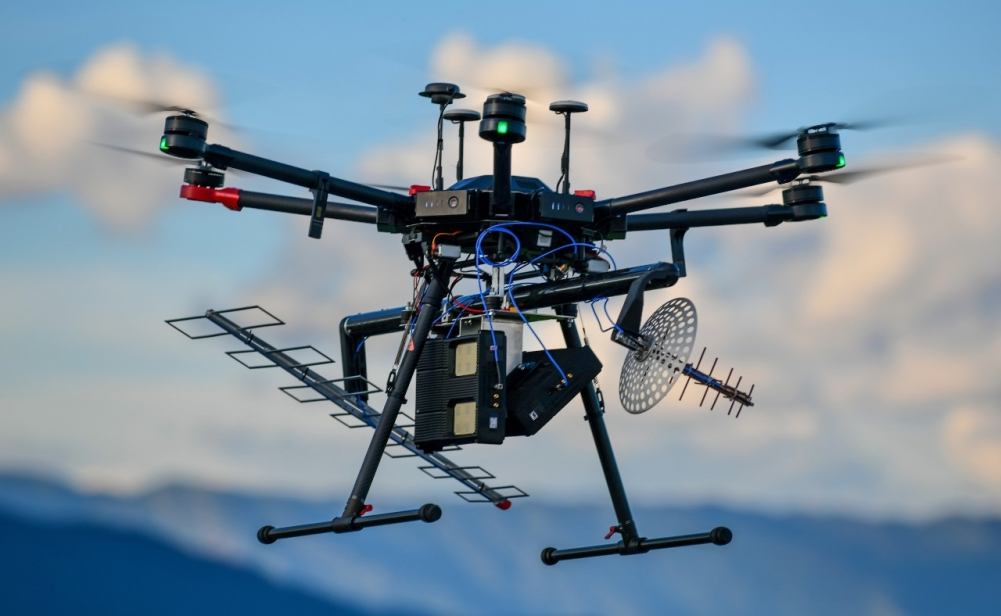
\includegraphics[width=.4\textwidth]{imgs_Joao/drone.jpg}
    \caption{Diversas aplicações se beneficiam do uso de drones e a obtenção de sua posição pode ser feita com receptores GNSS embarcados.}
    \label{fig:drone}
\end{figure}

\newpage

\noindent
\begin{tcolorbox}[colframe=black,width =7cm,colback=gray!20,arc=0pt]
\centering {\sc {\bf Exercícios Preparatórios}}
\end{tcolorbox}

\vspace{0.3cm}

\begin{enumerate}[label=$\blacktriangleright$ {\bf Exercício \arabic*},series=exerc,align=left]

\item {\bf (Parametrização das órbitas)} Cada constelação de satélites transmite informações distintas para descrição da órbita de seus satélites. No nosso modelo, vamos seguir as especificações do GPS e Galileo, que transmitem um conjunto de parâmetros chamados de \textbf{elementos orbitais de Kepler}, colocados na Figura \ref{fig:kep_orbit} (também recebem o nome de efemérides):
\begin{itemize}
    \item Excentricidade da órbita [$e$], que sempre vai ser um valor entre $0$ e $1$.
    \item Semieixo maior [$a$], metade da distância entre o apogeu e perigeu\footnote{\textit{apogeu}: ponto de maior distância entre satélite e terra, \textit{perigeu}: ponto de menor distância entre satélite e terra}
    \item Argumento do perigeu [$\omega$], define a orientação da elipse no plano orbital
    \item Inclinação [$i$], ângulo entre o plano equatorial da terra e o plano orbital
    \item Longitude do nó ascendente [$\Omega$], ângulo entre uma direção de referência e o nó ascendente\footnote{\textit{nó ascendente}: ponto no qual a trajetória do satélite cruza o plano orbital em sentido norte}
    \item Tempo desde o perigeu [$\Delta t$], tempo decorrido desde que o satélite passou pelo perigeu.
\end{itemize}

\begin{figure}[H]
    \centering
    \includesvg[width=.4\textwidth,inkscapelatex=false]{imgs_Joao/kep_orbit.svg}
    \caption{Elementos orbitais de Kepler}
    \label{fig:kep_orbit}
\end{figure}

Além desses parâmetros, usaremos o \textbf{parâmetro de gravitação padrão} da terra $\mu_\oplus = GM_\oplus$, sendo $G$ a constante da gravitação universal e $M_\oplus$ a massa da terra.

\begin{enumerate}[label=(\alph*)]
    \item (\textit{Parametrização da forma no plano orbital}) 
    
    Primeiramente, vamos começar descrevendo a elipse no sistema de coordenadas \textbf{perifocal}. Nesse sistema, a elipse está totalmente contida no plano, a origem está localizada no foco mais próximo ao perigeu, o eixo $x$ é orientado na direção do perigeu e o eixo $y$ com ângulo $\nu=90^\circ$, conforme a Figura \ref{fig:perifocal}.

    \begin{figure}[H]
        \centering
        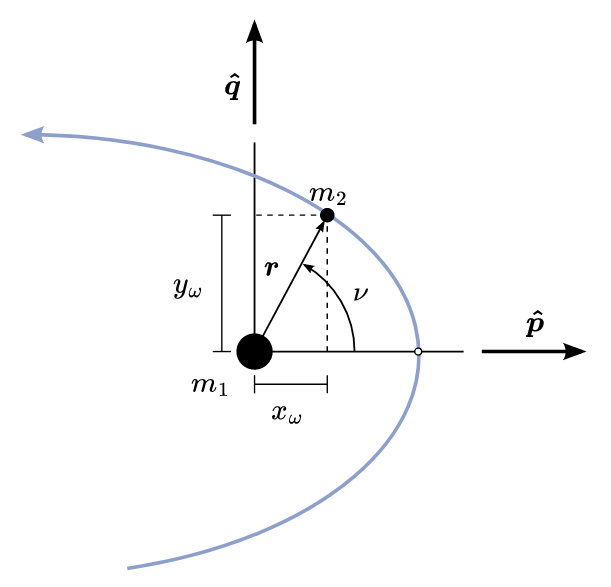
\includegraphics[width=.35\textwidth]{imgs_Joao/perifocal.png}
        \caption{Sistema de coordenadas perifocal}
        \label{fig:perifocal}
    \end{figure}

    Em primeiro lugar, escreva a parametrização cartesiana em termos de $r(t)$, distância entre o satélite e o centro da terra, e o ângulo $\nu(t)$, chamado de \textbf{anomalia verdadeira}.

    Em seguida, use um círculo auxiliar, de forma que a elipse fique circunscrita, e defina o ângulo central $E$ (\textbf{anomalia excêntrica}) como mostra a Figura \ref{fig:circumscribed}. Escreva a parametrização anterior em termos de $[E]$, $[a]$ e $[e]$.
    
    \begin{figure}[H]
        \centering
        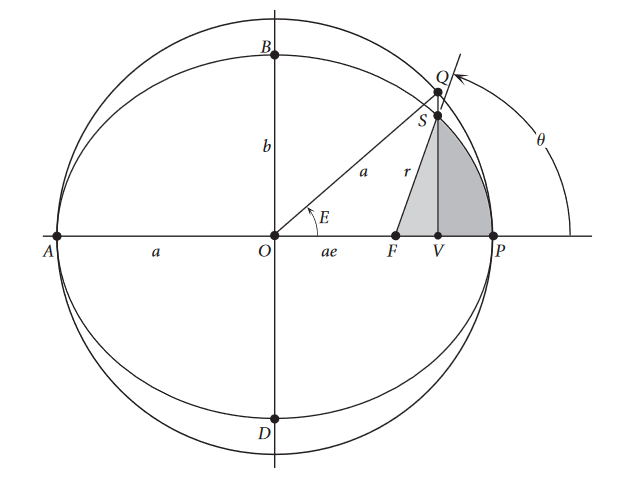
\includegraphics[width=.4\textwidth]{imgs_Joao/circumscribed.png}
        \caption{Elipse circunscrita e anomalia excêntrica}
        \label{fig:circumscribed}
    \end{figure}

    \item (\textit{Parametrização de tempo})

    Nesse próximo passo, a dependência temporal será incluída. Para simplificar as expressões, vamos definir a \textbf{anomalia média} como $M := \frac{2\pi}{T}\Delta t$, sendo $\Delta t$ o tempo desde o perigeu e $T$ o \textbf{período orbital}. 
    
    A dependência temporal da parametrização do item (a) é introduzida pela relação entre $E$ e $M$, dada pela \textbf{equação de Kepler}

    $$E(t) - e \sin E(t) = M(t)$$

    sendo $t$ o tempo atual.

    Desejamos então resolver a equação de Kepler, dado um valor de $M(t)$. No entanto, ela é uma \textbf{equação transcendente}. O que isso significa e qual a implicação disso?

    Abaixo segue um código de exemplo, que primeiro obtém uma solução para a equação de Kepler, em um instante $t$, e usa a solução para obter a posição no plano perifocal $(x_\omega, y_\omega)$. 

    \begin{minted}[
frame=lines,
framesep=2mm,
baselinestretch=1.2,
fontsize=\footnotesize,
]{python}
# Resolver equação de Kepler para E no instante t
E = resolve_kepler(t)

# Usar parametrização, usando valor de E(t)
xw = ... # Sendo x = x(E, a, e)
yw = ... # Sendo y = y(E, a, e)
    \end{minted}

    \item (\textit{Parametrização Espacial}) 
    
    Considerando agora a disposição espacial da órbita, desejamos escrever as coordenadas do sistema perifocal em um sistema \textbf{ECI} (\textit{Earth-Centered Inertial}). Em outras palavras, queremos descrever a órbita plana no espaço tridimensional.
    
    Para isso, três rotações sucessivas são necessárias (Figura \ref{fig:rotations}):
    \begin{enumerate}
        \item Rotacionar em torno $z_\omega$, até que o eixo $x_\omega$ esteja alinhado com o nó ascendente,
        \item Rotacionar em torno do novo $x_\omega'$, até que o plano orbital e equatorial estejam alinhados,
        \item Rotacionar em torno de $z'$, para alinhar o nó ascendente com a direção de referência.
    \end{enumerate}

        \begin{minted}[
frame=lines,
framesep=2mm,
baselinestretch=1.2,
fontsize=\footnotesize,
]{python}
# Obtém matriz de rotação
ângulos = ... # Os ângulos associados as rotações descritas em i, ii e iii
ordem_rotação = "ZXZ"
R = rotaciona(ordem_rotação, ângulos)

pos3d = R @ posPerifoc   # Rotaciona o vetor em coorenadas perifocais, posPerifoc = [xw, yw, 0]
# @ é o operador de multiplicação matricial
    \end{minted}

    \begin{figure}[H]
        \centering
        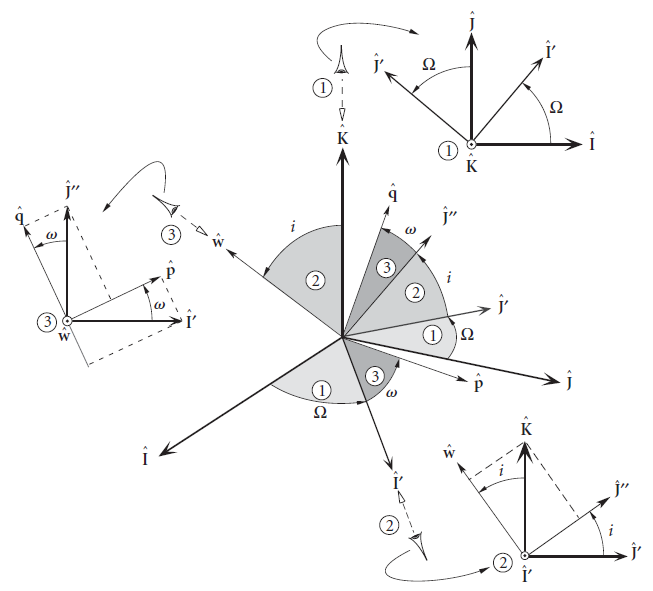
\includegraphics[width=.4\textwidth]{imgs_Joao/rotations.png}
        \caption{Rotações para alinhar os ângulos}
        \label{fig:rotations}
    \end{figure}
\end{enumerate}

\item {\bf (Trilateração e Gradiente Descendente)} A partir de um conjunto de medidas de distância com relação a diferentes transmissores, um receptor pode estimar sua posição resolvendo um problema geométrico de intersecção de círculos (ou esferas), como exemplifica a Figura \ref{fig:trilateration}. Para resolver esse problema, os seguintes itens são necessários:
\begin{itemize}
    \item A posição de cada um dos satélites (não é mais um problema graças ao \textbf{Exercício 1})
    \item As distância relativas para cada um dos satélites
    \item Equacionar cada uma das leituras
    \item Resolver o sistema de equações resultante
\end{itemize}

\begin{figure}[H]
    \centering
    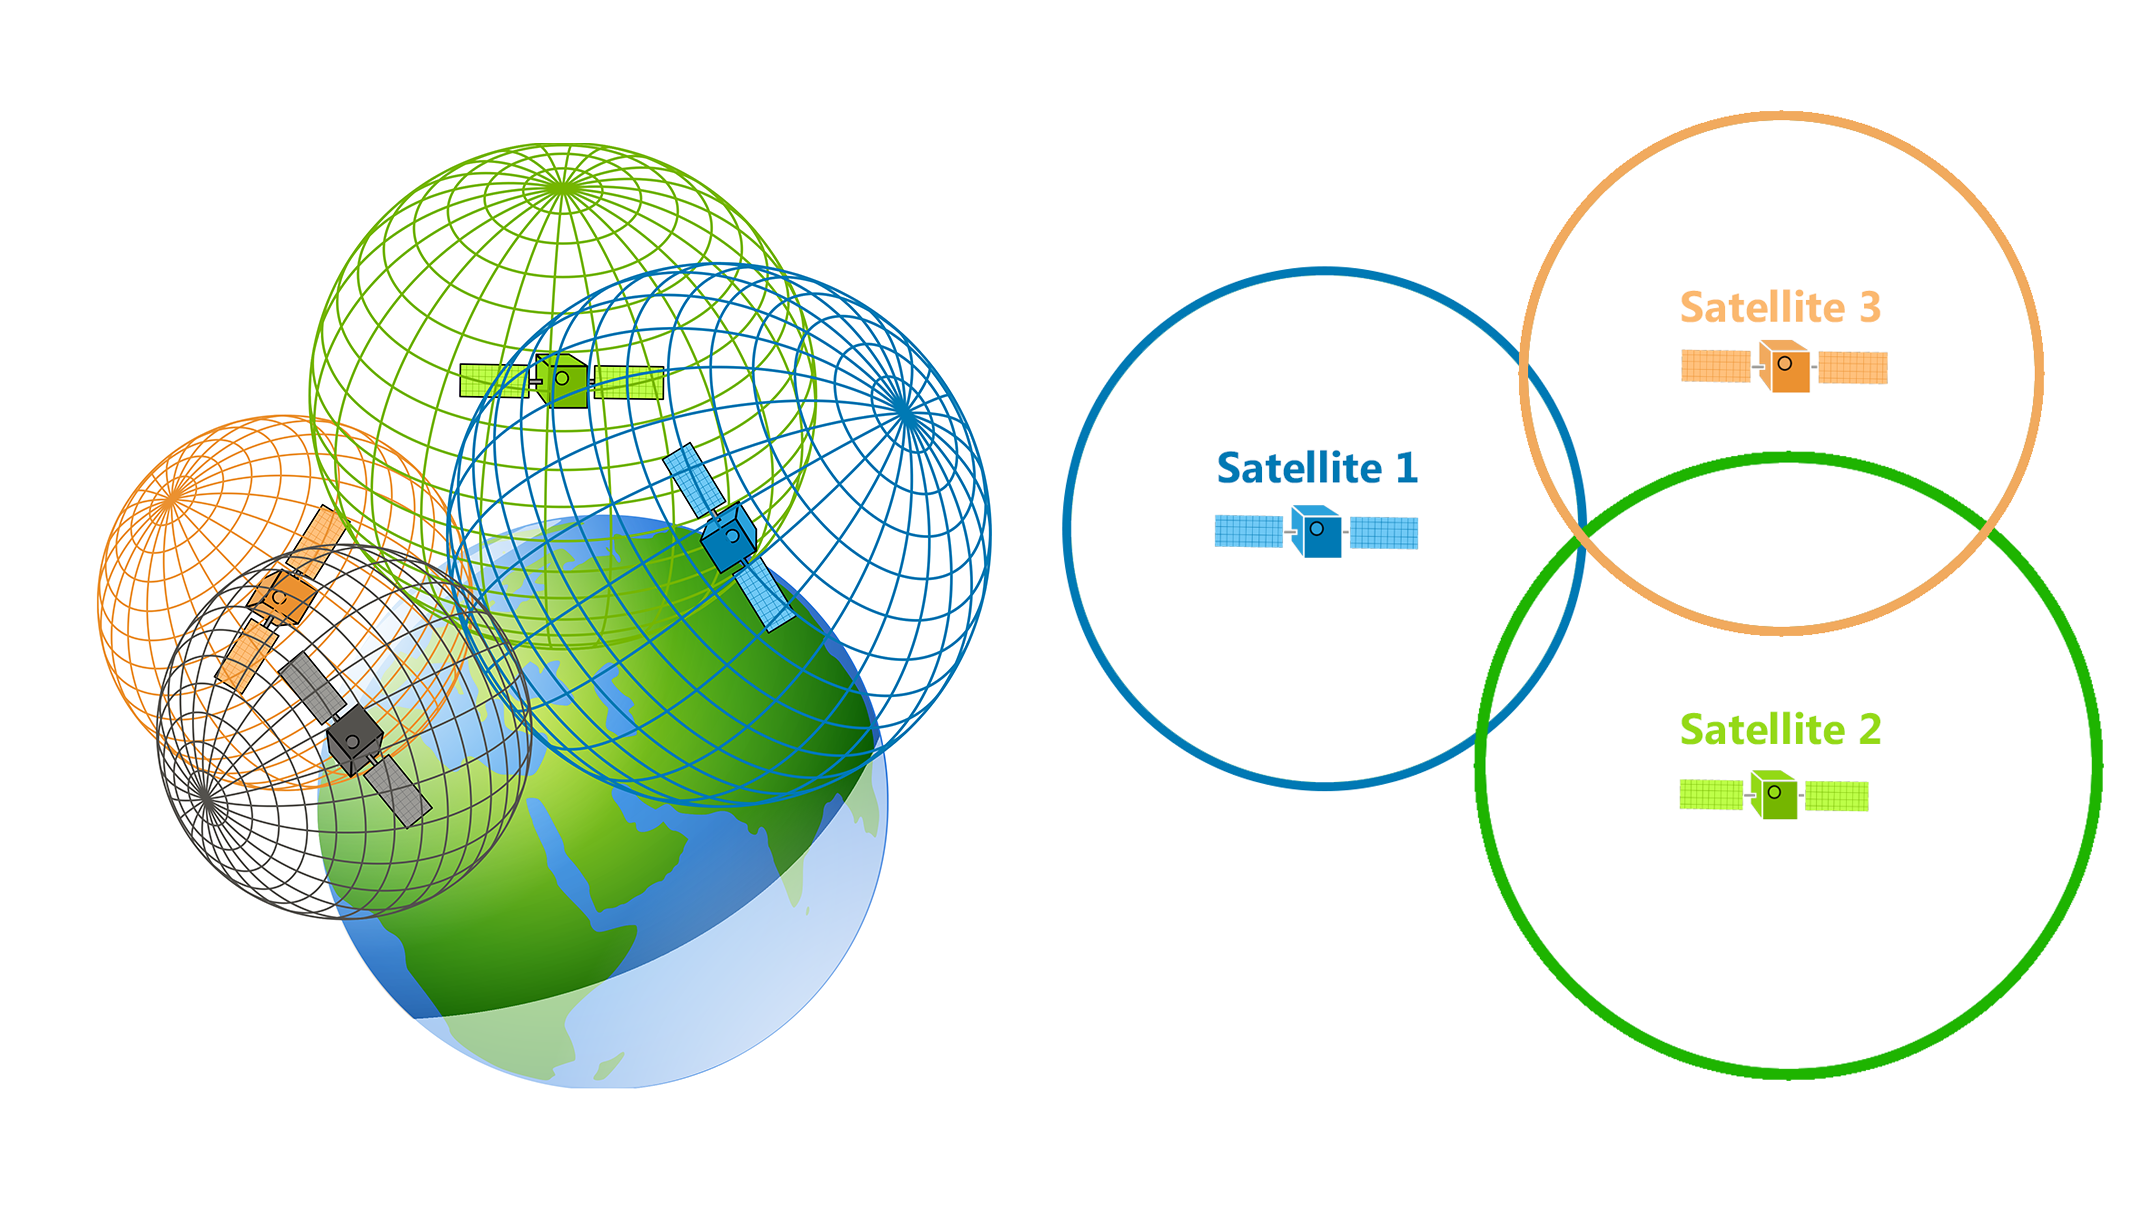
\includegraphics[width=.5\textwidth]{imgs_Joao/trilateration.png}
    \caption{Múltiplos satélites medem distâncias relativas com relação ao receptor.}
    \label{fig:trilateration}
\end{figure}

\begin{enumerate}[label=(\alph*)]
    \item (\textit{Medidas de Distância}) 
    
    A partir da leitura do \textbf{TOT} (\textit{time of transmission}), codificado no sinal do satélite, e do relógio interno, indicando o \textbf{TOA} (\textit{time of arrival}), o receptor é capaz de determinar o TOF (\textit{time of flight}). Além disso, com essa última informação, ele é capaz de calcular a distância relativa para esse satélite.

    Explique esse procedimento. 
    
    \item (\textit{Sistema de Equações}) 
    
    A partir das medidas de distância $\rho_i$ (distância entre satélite $i$ e receptor) e da posição $\mathbf{r}_i$, obtenha o sistema de equações. O que se pode afirmar sobre a linearidade desse sistema de equações?

    \item (\textit{Encontrando Soluções})
    
    Além da natureza do sistema obtido, todas as medidas de GNSS apresentam erros e, portanto, pode ser que não exista uma solução. Dessa maneira, diversas técnicas se apoiam em \textbf{soluções iterativas} nesses cenários (como vimos no Exercício 1(b)), que buscam otimizar determinado critério.
    
    Por exemplo, ao usar uma função $J(\theta)$ de critério, dependente de uma possível solução $\theta$, que assume valores maiores para soluções piores e valores menores para as melhores, o problema consiste em encontrar o valor de $\theta$ que minimiza essa função (a melhor solução possível). A notação para esse tipo de problema é:

    $$\hat{\theta} = \argmin_\theta J(\theta)$$
    
    Um critério possível no problema da localização do drone é uma função $J(\mathbf{r})$ que depende de um ``chute'' inicial de posição, $\mathbf{r}$, e avalia a diferença entre a medida e o valor calculado usando o chute. Uma função $J$ possível seria

    $$J(\mathbf{r}) = \frac{1}{2}\sum_{i=1}^{N}\left(\|\mathbf{r}_i - \mathbf{r}\|^2 - \rho_i^2\right)^2$$

    para um conjunto de $N$ medidas. 
    
    A partir da Figura \ref{fig:trilateration}, qual o valor de $J$ quando escolhemos a posição certa do receptor (desconsiderando os erros na medida)? O que podemos dizer sobre o valor de $J$ para outros valores de $\mathbf{r}$? 
    
    \item (\textit{Gradiente Descendente})

    \textbf{Problemas de otimização}\footnote{A página da Wikipedia sobre otimização merece um tour: \url{https://en.wikipedia.org/wiki/Mathematical_optimization}} são ubíquos nas diversas áreas da ciência e engenharia e, em problemas de natureza contínua, é possível usar os conceitos de análise vetorial vistos na disciplina para obter boas soluções.

    Nesse sentido, o conceito do \textbf{vetor gradiente} $\nabla f$, de uma função multivariável $f: \R^n \to \R$ em um ponto $\mathbf{x}\in \R^n$, é especialmente útil uma vez que ele indica a direção de máxima subida e máxima descida (\textit{Problema 3 e Problema 4, Lista 3}). Portanto, o gradiente de uma função que se deseja maximizar/minimizar vai indicar o melhor caminho local.

    Usando essas ideias, descreva um método iterativo de otimização que use o gradiente e demonstre como ele pode ser aplicado para o problema de \textbf{trilateração}:

    $$\argmin_\mathbf{r} \frac{1}{2}\sum_{i=1}^{N}\left(\|\mathbf{r}_i - \mathbf{r}\|^2 - \rho_i^2\right)^2$$

\end{enumerate}

\end{enumerate}


\vspace{0.3cm}

%\begin{multicols}{2}

\noindent
\begin{tcolorbox}[colframe=black,width =7cm,colback=gray!20,arc=0pt]
\centering {\sc {\bf Projeto}}
\end{tcolorbox}

O objetivo do projeto é implementar um programa que seja capaz de determinar a posição de um drone em múltiplos instantes de tempo, a partir dos dados fornecidos por um receptor GNSS embarcado.

O programa pode ser implementado em qualquer linguagem e as especificações são:
\begin{enumerate}[label=\Roman*)]
    \item Deve ser capaz de resolver as posições dos satélites, considerando que as informações obtidas pelo receptor seguem as especificações do \textbf{Exercício 1}.
    \item Deve ser capaz de estimar a posição do drone em um instante de tempo, com o método discutido no \textbf{Exercício 2}.
\end{enumerate}

A implementação deve ser original, mas é permitido o uso de funções e módulos auxiliares para passos intermediários. Não é permitido usar bibliotecas que satisfaçam, em totalidade, as especificações I e/ou II.\footnote{Em caso de dúvidas sobre as restrições, entre em contato.}

\vspace{0.3cm}


%\end{multicols}
\end{document}




